\documentclass[a4paper,12pt]{article}

\usepackage[T1,T2A]{fontenc}        % Кодировки шрифтов
\usepackage[utf8]{inputenc}         % Кодировка текста
\usepackage[english,russian]{babel} % Подключение поддержки языков

\usepackage{amsthm}                 % Оформление теорем
\usepackage{amstext}                % Текстовые вставки в формулы
\usepackage{amsfonts}               % Математические шрифты

\newtheorem*{ther}{Теорема}
\newtheorem*{defi}{Определение}

\newcommand{\eps}{\varepsilon}
\usepackage{graphicx}

\begin{document}

    \section*{Задача 23}
    
    Дайте определения эквивалентных функций, бесконечно малой функции и функций одного порядка. Найдите функцию $g(x) = Cx^a$, эквивалентную функции $f(x)= \sqrt[3]{x^6+3\sqrt[5]{x}}$, при х -> 0, x -> inf.
    
    \subsection*{Решение}
    
    \begin{defi} бесконечно малые функции a(x) и b(x) называются эквивалентными бесконечно малыми при х->a, если
    $\displaystyle \lim_{n\rightarrow a}
                   \frac{a(x)}{b(x)}
                   =1
    $ 
    \end{defi}
    \begin{figure}[h!]
    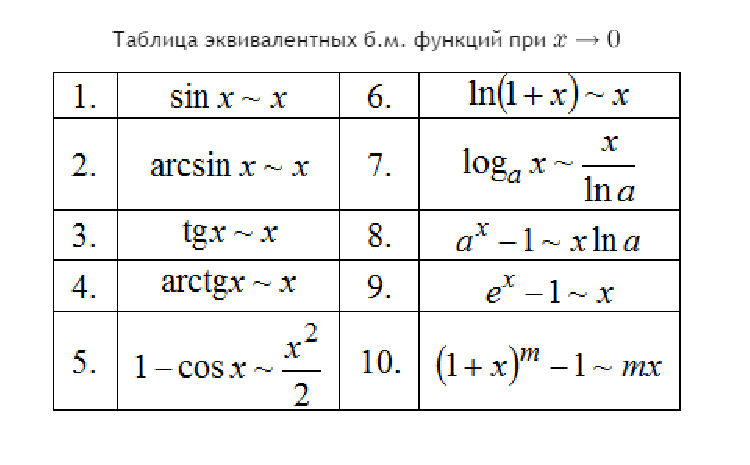
\includegraphics[width=1\linewidth]{_PNG}
    \end{figure}
    \clearpage
    \begin{defi}  функции a(x) и b(x) называются бесконечно малыми одного порядка малости при х->a, если
    $\displaystyle \lim_{n\rightarrow a} 
                   \frac{a(x)}{b(x)}
                   =c, c != 0
    $              
    
    \end{defi}
    \begin{defi} функция y = f(x) называется бесконечно малой при x -> a, если
    $\displaystyle \lim_{n\rightarrow a} 
                   f(x) = 0
    $
                 
    \end{defi}
    
    \textbf{Примеры:}
        \begin{enumerate}
            \item $f(x) = (x-1)^2$ -- бесконечно малая при х -> 1.
             \item $f(x) = \frac{1}{x}$ -- бесконечно малая при х -> $inf$.
        \end{enumerate}
   
    
        \subsection*{Задание}
        Найдите функцию $g(x) = Cx^a$, эквивалентную функции $f(x)= \sqrt[3]{x^6+3\sqrt[5]{x}}$, при х -> 0, x -> inf.
            \begin{enumerate}
                \item x -> 0. Рассмотрим g(x) = $\sqrt[3]{3}\cdot\sqrt[15]{x}$
                
                $\displaystyle \lim_{n\rightarrow 0} 
                   \frac{
                       \sqrt[3]{x^6+3\cdot \sqrt[5]{x}}
                   }
                   {
                   \sqrt[3]{x^6+3\sqrt[5]{x}}
                   }
                   =
                   \displaystyle \lim_{n\rightarrow 0} 
                   \frac{
                       \sqrt[3]{\frac{x^6}{x^{1/5}} + 3 \cdot \frac{x^{1/5}}{x^{1/5}}}
                   }
                   {
                   \sqrt[3]{3}
                   }
                   =
                   \displaystyle \lim_{n\rightarrow 0} 
                   \frac{
                       \sqrt[3]{x^{29/5} + 3}
                   }
                   {
                   \sqrt[3]{3}
                   }
                   = 
                   1
    $    
                \item Это значит, что g(x) - искомая эквивалентная функция.
                
                \item x -> inf, положим g(x) = $x^2$
                $\displaystyle \lim_{n\rightarrow \infty} 
                   \frac{
                       \sqrt[3]{x^6+3\cdot \sqrt[5]{x}}
                   }
                   {
                   x^2
                   }
                   =
                   \displaystyle \lim_{n\rightarrow \infty} 
                       \sqrt[3]{1 + 3 \cdot x^{-29/5}}
                   = 
                   1
    $    
        \item А значит, g(x) - искомая эквивалентная функция. Мы красавы!
            \end{enumerate}
\end{document}